\chapter{Background and History\label{section:history}}
\section{Background}\label{section:background}
In this section we will cover all the necessary information to understand this
thesis. We will start on a high level and slowly delve deeper into the
intricacies of a camera.

\subsection{Camera}
Before we delve deeper, what is a camera? In this section we will cover a brief
and incomplete history of cameras followed by an explanation of how modern
cameras work. In the simplest of terms, a camera is just a box with a tiny
hole. This box with the tiny hole is called the \textit{Camera Obscura}, which
is a natural phenomenon where light enters a small hole into a dark box the
light will be projected upside down to the opposing wall. This discovery goes
back to the Chinese philosophers of the fifth century BC. The first record of
seeing an inverted image when looking through a pinhole was by the philosopher
Mo Ti\cite{hammond1981camera} (aka. Mozi). This was the very basics of a
camera, it was another four centuries before Tuan Chheng Shih took another
crack at this. He realized that the image was inverted because, like an oar;
when the oar is up, the blade is down. In the west, Aristotele had also seen
this phenomenon. Observations made by the Chinese and the greek are very close,
to the extent that it is unclear if they were made independently or if there
was collaboration. In \cref{fig:cameraobscura} we can see an example of how
this system looks like. The light comes and flips it around. This is the basis
of cameras.

Jumping ahed to the 13th century, Roger Bacon began working with the camera
obscura. He described a way to create an aerial image using a mirror infront of
the aperture\footnote{The hole in the "camera"} so that an observer would not
see anything. For example to view on people walking underneath a window.

This was only the first part though, by the 18th century people had largely
figured out what camera obscuras were. Lenses existed to create a clearer
projected view. The part that was left was to actually store the light onto
something. In 1725 Johann Heinrich Schulze observed that when silver salts
were exposed to light, they darkened. Contrary to what people believed at the
time he showd that it was due to light alone, not the air or the
sun~\cite{gernsheim1986concise}. After much experimentation based on this
discovery, a French inventor named Nic\'ephore Ni\'epce figured out how to
then capture an image. This image was the view of his window taken onto a
pewter plate~\cite{gernsheim1986concise}. Today silver chloride is no longer
used in cameras, we do not need to produce negatives of images to produce an
image. Instead we use photodiodes, these are diodes that can convert light to
electricity. We will cover modern sensor technologies in \cref{section:sensortechnology}.

So how do all of these tie into modern cameras, the mirror design that Roger
Bacon designed is now in use in devices such as DSLRs when using the viewfinder
window. When pressing down the shutter, the mirror flips down which is why when
taking a picture the viewfinder goes blank for a bit. This allows the sensor to
receive light, which the photodiodes then turn into electricity. After the
sensor receives light, it gives the image data to the \textit{Image Signal
Processor} (ISP), the ISP is covered in detail in \cref{section:isp}. When
using the viewfinder in a screen, the mirror is put down and light is given to
the sensor. The ISP then processes this image and spits out a lower quality
image for preview. As mobile phones do not have physical viewfinders, this is
what mobile phones then use.

\begin{figure}
    \centering
    \subfloat[Camera obscura]{
        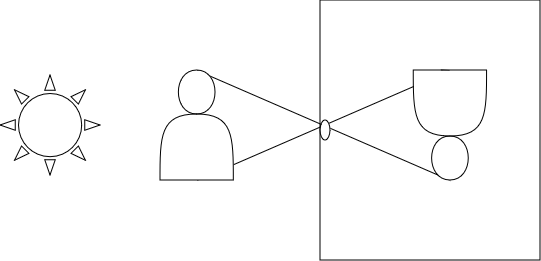
\includegraphics[width=0.5\textwidth]{figures/camera obscura.png}
        \label{fig:cameraobscura}
    }
    \subfloat[Worlds first image~\cite{gernsheim1986concise}]{
        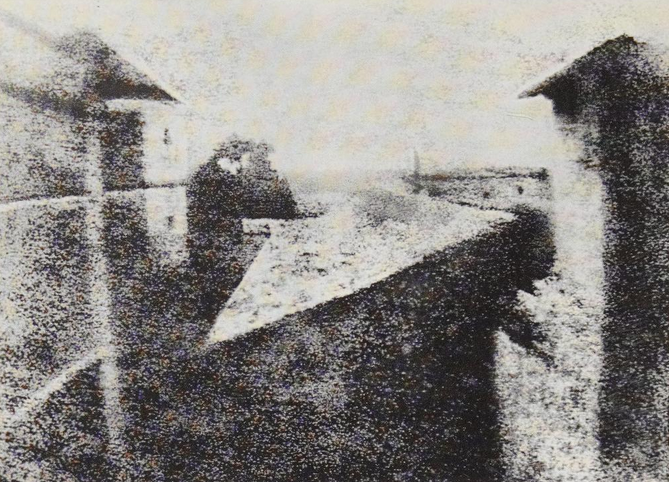
\includegraphics[width=0.4\textwidth]{figures/worldsfirstimage.png}
        \label{fig:worldsfiristimage}
    }
    \qquad
    \subfloat[A DSLR camera]{
        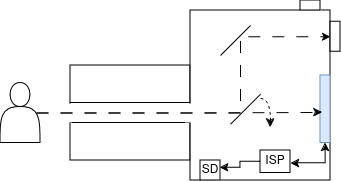
\includegraphics[width=0.4\textwidth]{figures/camera.png}
        \label{fig:camera}
    }
    \caption{}
\end{figure}


\subsection{3D cameras}
In fields like robotics 3D cameras are used, this allows the robots to get a
sense of depth. There are many different technologies that are used for getting
depth, such as \textit{Light Detection And Ranging} (LiDAR), stereo
cameras and more. We will give a brief overview of how some of these
technologies work.

\textbf{LiDAR} as the name suggests, works using light ($c$), specifically
lasers. It measures distance ($d$) by measuring the time ($t$) it takes for the
light to travel to the object and back.
\[
    d = \frac{c \cdot t}{2}
\]
If the laser hits for example a mirror, an object that reflects the light
elsewhere, the distance measurement may be inaccurate. There is some work that
has been done in order to improve the accuracy of measurements on these
surfaces~\cite{foster2013visagge, henley23lidar}. While the technology has come
a long way, often a secondary sensor technology is accompanied with LiDAR for
detecting specular surfaces such as ultrasonic scanners~\cite{diosi2004advanced}.

\textbf{Stereo cameras}, like human eyes uses two cameras next to eachother.
By taking two images depth can be calculated~\cite{adi2017distance}. It is done
by finding the same point in the two images, this is a well known problem~
\cite{scharstein2002taxonomy}. There are several solutions to this problem,
a simple one is the absolute difference in color. While we will not delve
deeper into the algorithms here, a detailed comparison can be read from~\cite{scharstein2002taxonomy}.

\subsection{Sensor technology}\label{section:sensortechnology}
At its core, sensors are just some photodiodes that can convert photons
into electrical charge. In this section we will cover two common sensor this is
done.

There are multiple types of photodiodes, though the idea behind them is to
create voltage out of photons that hit them. It does this using a
\textit{positive-negative}(PN) junctions, a junction made of one positive and
one negative material that do not fill all of the electron slots in the atom.
This allows electrons to then flow freely, allowing the charge to
move~\cite{peterson2001works}.

\subsubsection{Complementary Metal Oxide Semiconductor Sensors}
\textit{Complementary Metal Oxide Semiconductor} (CMOS) sensors are very old
sensors, being around since the 1960s~\cite{ieeeCMOS}. Over the years due to
lithography improvements they have become very good, being able to compete with
with \textit{Charged Couple Device} (CCD) sensors which are known for better
image quality technology~\cite{ieeeCMOS}. While CCDs have a better image quality, it requires
much more power than CMOS which can be up to 100 times less power hungry~
\cite{CMOSReview}. This means that in many mobile devices and other low power
devices wants CMOS over CCDs.

CMOS sensors are similar to the CMOS memory chips, unlike the memory chips the
sensors use photodiodes along with amplifiers (\cref{fig:cmosvsccd}) over
transistors. The amplifiers exist to, well, amplify the signal. This design
allows us to access individual pixels quickly, see \cref{fig:ccdbloom} using
random access on top of being able to read out R, G and B signals
simultaneously~\cite{cmosAlen}. Because there are so many photodiodes along
with amplifiers, electrical fluctuation is created. This causes intermittencies
in the quality of the image, there are a number of noise reduction algorithms
that can be applied on the image to remove these.

Curious readers can have a look at \cite{CMOSReview, ieeeCMOS} for a more
in depth overview of what CMOS sensors are.

\subsubsection{Charged Couple Device Sensors}
\textit{Charged Couple Device} (CCD) sensors were for a long time considered
significantly better than CMOS~\cite{ieeeCMOS}. It works using capacitors next
to the photodiodes to create voltage out of charge which is then read out in a
serial manner. Unlike CMOS, CDD allows you to design very small pixel sizes as
the pixels themselves do not require much real estate. The downside of this is
that this creates a lot of heat, requiring good cooling~\cite{meng2016numerical}
which is not always available in devices such as mobile phones. In
\cref{fig:cmosvsccd} we can see how the CCD sensor looks like on a high level.
Because CCD sensors read the signals row by row, if there are some pixels are
very bright it can create visual effects for the entire row~\cite{ieeeCMOS} as
can be seen in \cref{fig:ccdbloom}.

\begin{figure}
    \centering
    \subfloat[CCD blooming effect,\\\textit{image source: \href{https://en.wikipedia.org/wiki/Charge-coupled\_device}{Wikipedia}}]{
        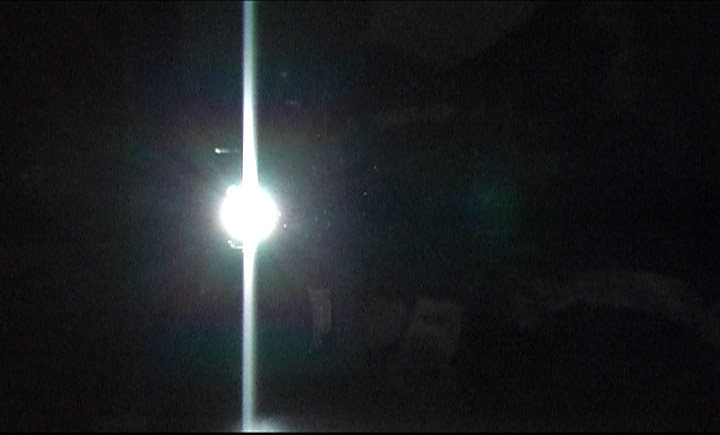
\includegraphics[width=0.40\textwidth]{figures/ccd_blooming.jpg}
        \label{fig:ccdbloom}
    }
    \subfloat[CMOS vs CDD comparison~\cite{ieeeCMOS}]{
        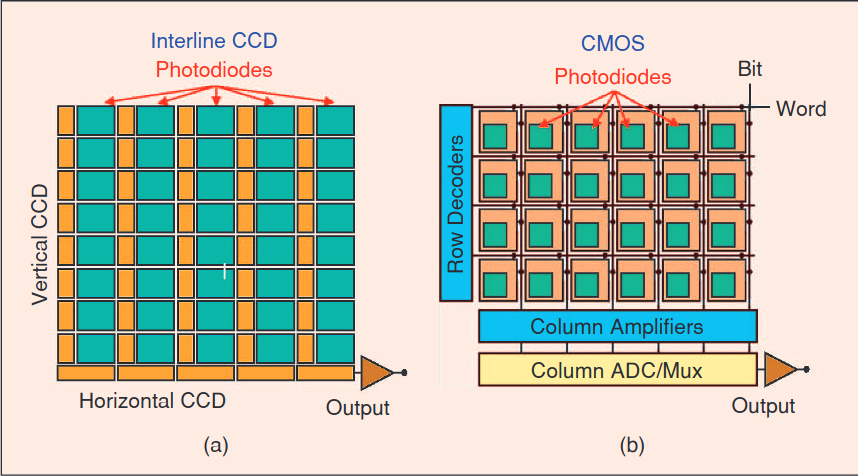
\includegraphics[width=0.5\textwidth]{figures/cmos_vs_cdd}
        \label{fig:cmosvsccd}
    }
    \caption{}
\end{figure}

\subsection{Image Signal Processors} \label{section:isp}
\textit{Image Signal Processors} (ISPs) are a highly secretive piece of
hardware\cite{adams2010frankencamera}. There are few systems that say they even
have one, and even fewer that explain how they work. To understand how ISPs
work, we will be using the Raspberry
Pi\footnote{https://datasheets.raspberrypi.com/camera/raspberry-pi-camera-guide.pdf}
\footnote{https://datasheets.raspberrypi.com/camera/raspberry-pi-image-signal-processor-specification.pdf},
it is the only one that is open source (except for the \textit{Register
Transfer Level} (RTL) code) along with an open specification. RTL code is the
abstraction for how hardware is designed. It is the way to program how the
wiring should look like in the actual chip.

In this section we will give an overview of what ISPs typically do and how they
function. Though ISPs can differ slightly though the idea is roughly the same
across the board.

So ISPs, what exactly are they? As the name suggests, they process image
signals. When an image come from the sensor the signal (image) contains a lot
of redundant and unprocessed information. The sensor is also also not quite
calibrated to the real world environment, a lot of things are simply wrong with
it. For example, if a sensor was hardcoded to a certain light level, it would
look very dark once a cloud blocked the sun. Correcting these issues is an
expensive process, so much so that there is a hardware block in camera systems
that does this for you.

The isp has a couple steps (highly hardware dependant, for specifics see the
manual if it exists), most work something along the lines of

\begin{figure}[htpb]
    \centering
    \subfloat[Blue Channel]{
        
\includegraphics[width=0.2\textwidth]{figures/bayer_frame_blue.png}
        \label{fig:bayer_blue}
    }
    \qquad
    \subfloat[Green Channel]{
        
\includegraphics[width=0.2\textwidth]{figures/bayer_frame_green.png}
        \label{fig:bayer_green}
    }
    \qquad
    \subfloat[Red Channel]{
        
\includegraphics[width=0.2\textwidth]{figures/bayer_frame_red.png}
        \label{fig:bayer_red}
    }
    \qquad
    \subfloat[Full Bayer Frame]{
        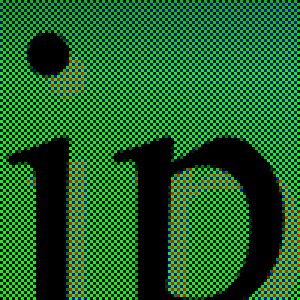
\includegraphics[width=0.2\textwidth]{figures/bayer_frame.png}
        \label{fig:bayer_full}
    }
    \qquad
    \subfloat[Final image]{
        
\includegraphics[width=0.2\textwidth]{figures/bayer_final}
        \label{fig:bayer_final}
    }
    \qquad
    \subfloat[Bayer pattern]{
        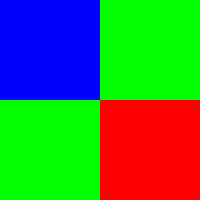
\includegraphics[width=0.2\textwidth]{figures/bayerpattern.png}
        \label{fig:bayer_pattern}
    }

    \caption[Bayer demosaicing]{Bayer demosaicing, \textit{source: https://en.wikipedia.org/wiki/Demosaicing}}
    \label{fig:bayer_channels}
\end{figure}

\begin{enumerate}
    \item Receive raw sensor data, often a Bayer image or similar

    \item The ISP then begins applying the autocontrol algorithms, the standard
        ones are known as the \textit{Tripple autocontrol} (3A) algorithms for
        auto white balancing, gain, and focus control\cite{libcameraStack}. These will be covered
        in a bit more detail in \cref{section:autocontrol}.

    \item Demosaic the image, i.e. extracting the pixel data from the raw
        image. The is often done using a Bayer like filter, many exist though
        they all work in the same way. In \cref{fig:bayer_channels} we can see
        how each of these channels are extracted. Once extracted they are
        combined into the final image as seen in \cref{fig:bayer_final}~\cite{li2008image, libcameraStack}. One
        way this can be done is taking the average of each nearby pixel and
        interpolating them into a single one. This is quite crude compared to
        the real thing but the idea is the same. \cref{fig:bayer_pattern}

    \item After processing the image in the ISP, the ISP then gives the image
        to the application that requested the image. The ISP also re-calibrates
        the autocontrol parameters based on the ones that were computed for the
        current frame. This is in order to correct for example white balancing,
        if coming from a very dark room into a very light room, it uses the
        current parameters to improve the white balancing.

\end{enumerate}

Depending on the hardware, the 3A can be done using raw images or not.

\subsubsection{Autocontrol algorithms} \label{section:autocontrol}

When people talk about their images being unedited, most do not realize that all
photos are edited to a degree. Some better than others, autocontrol algorithms
today can process an image quite heavily. This section will give an overview of
what autocontrol algorithms are, though not the inner workings of these
algorithms.

Effectively all ISPs today implement at the very least the 3A (\textit{Auto
White Balancing} (AWB), and \textit{Auto Gain Control} (AGC), \textit{Auto
Focus Control} (AFC)) algorithms. When the ISP receives metadata from the
sensor, it uses the AFC algorithm to focus on a specific object that the user
tries to focus on. Similarly, the AGC algorithm is used to make sure that the
image wll not be too bright or dark. AWBs purpose on the other hand is to make
sure that the temperature of the image is correct. Blue being cold and yellow
being warm, it balances the whites to reflect reality as closely as possible.

On top of the 3A algorithms, there are a lot more that the ISP often does. For
example there is often some vignetted, color correction and more. In
\cref{fig:lens_shading} we can see an example of how the ISP has fixed the image.
In \cref{fig:with_shading} the corners are significantly darker than the center.
While in \cref{fig:without_shading} the whole image is equally lit.

\begin{figure}[htpb]
    \centering
    \subfloat[With vignette]{
        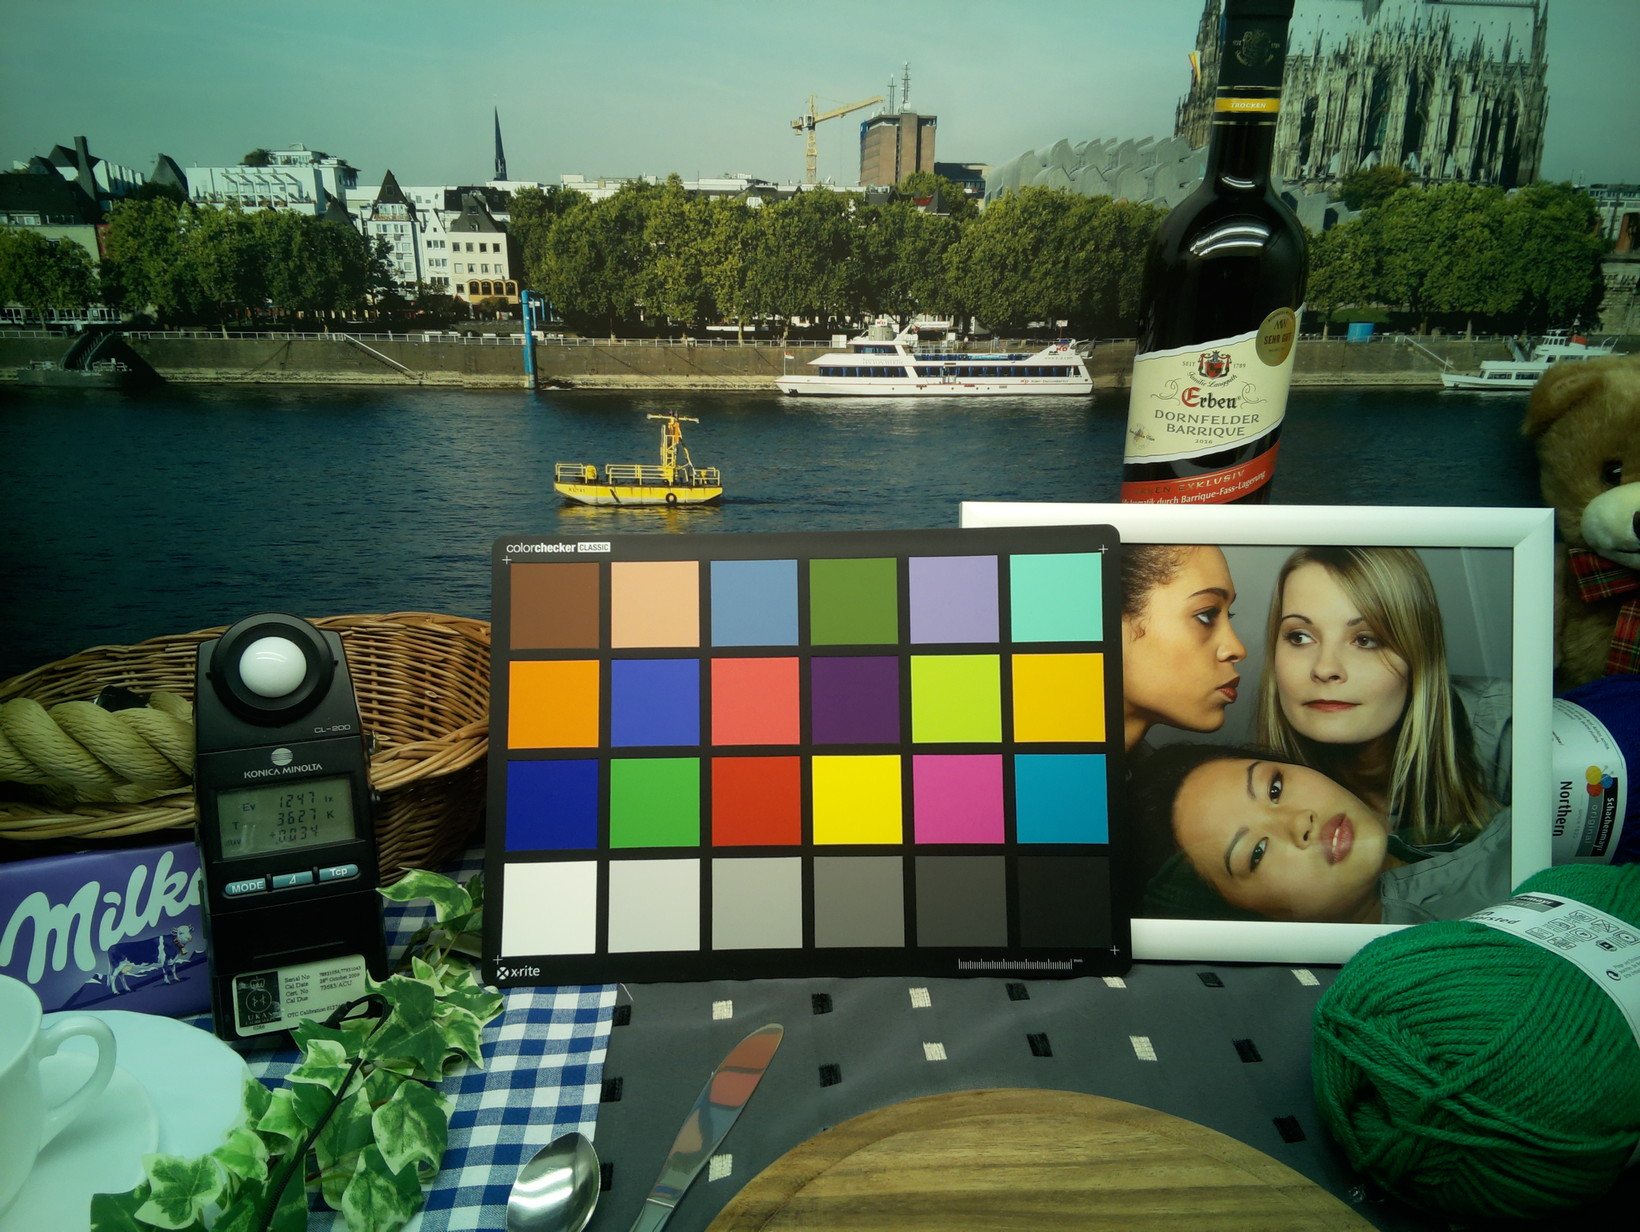
\includegraphics[width=0.4\textwidth]{figures/alsc-none.jpg}
        \label{fig:with_shading}
    }
    \qquad
    \subfloat[Without vignette]{
        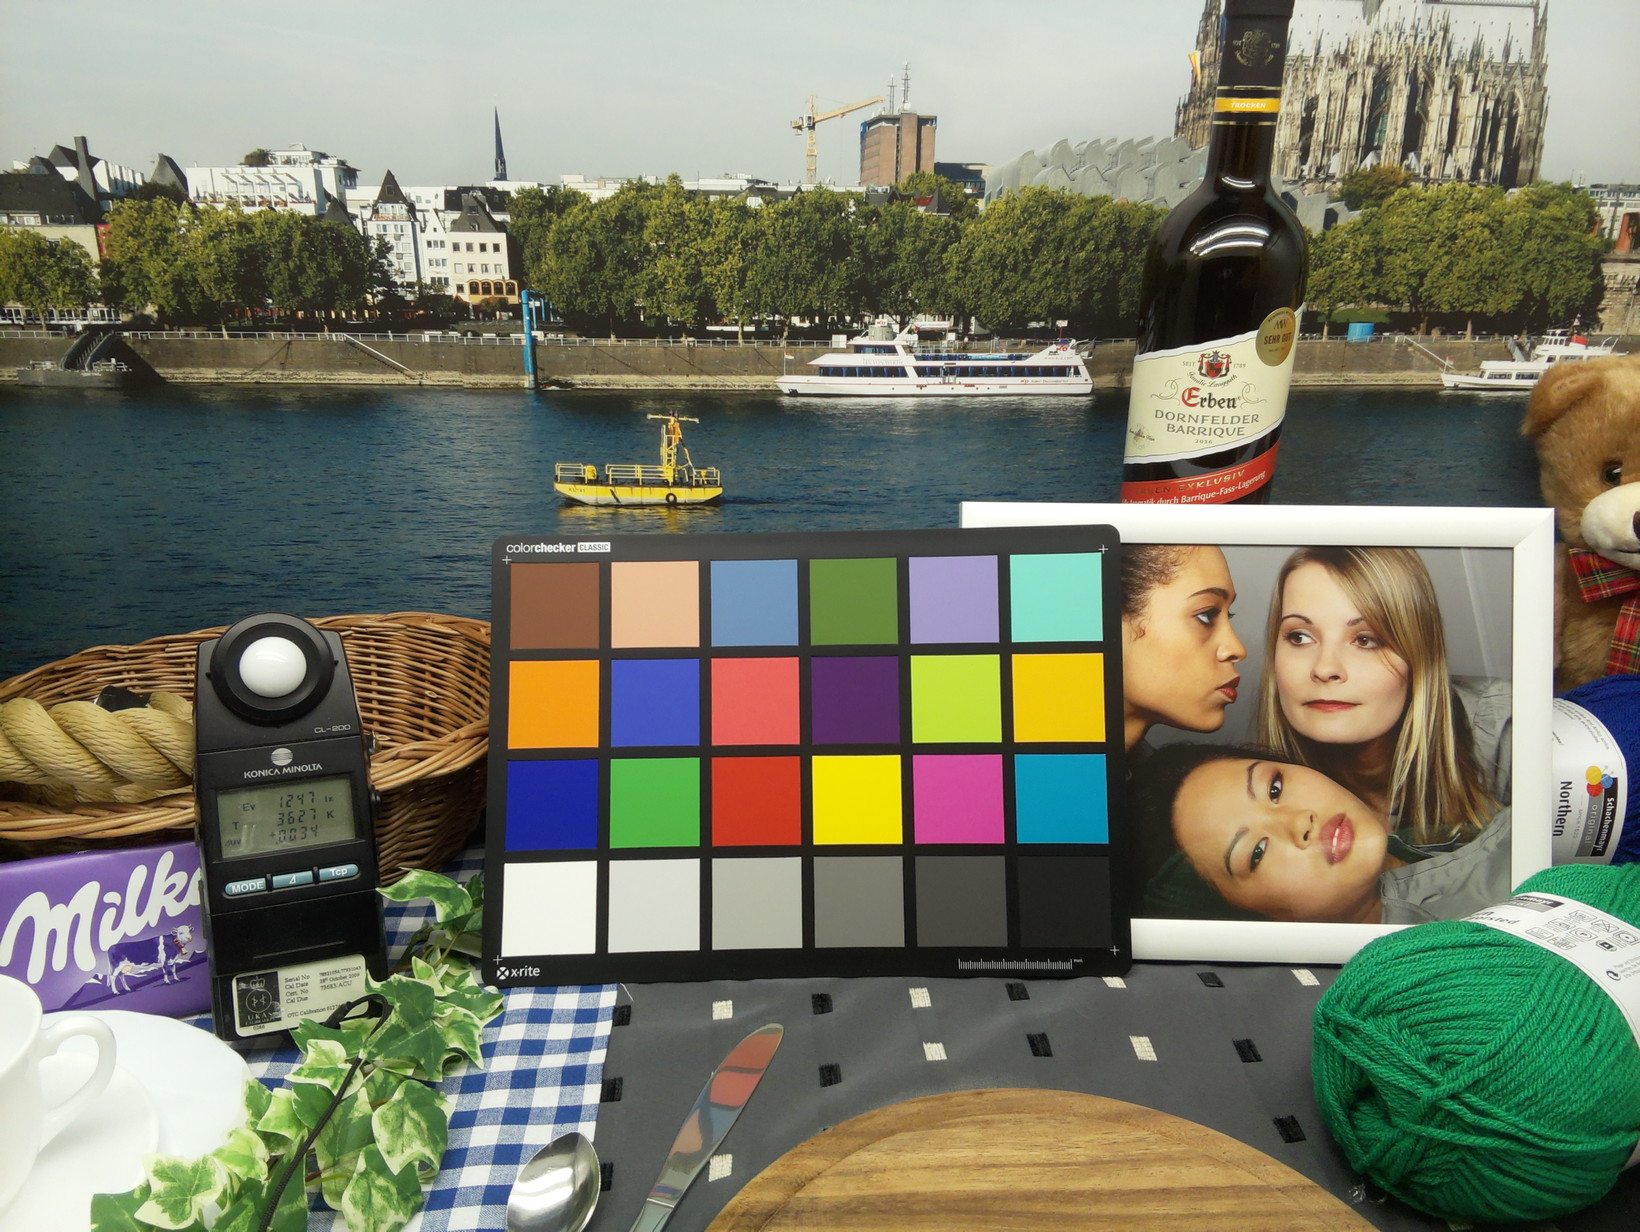
\includegraphics[width=0.4\textwidth]{figures/alsc-both.jpg}
        \label{fig:without_shading}
    }

    \caption{Different lens shading corrections. \textit{Photo by Naush Patuk used with permission}}\label{fig:lens_shading}
\end{figure}

\subsubsection{Image Processing and Tiles}
The Raspberry Pi ISP is divided into two sections, the front- and back end.
Though the front end has some image processing capabilties, being able to scale
and crop images. Its main responsibility is to write images to main memory,
providing an
AXI\footnote{https://developer.arm.com/documentation/ihi0051/latest} interface
to give the ISP frames. While doing this, it provides the backend with some
statistics of the image. These statistics consist of for example histograms
of color counts etc.

The backend then reads these images that the frontend has provided. Unlike how
applications deal with full frames, the backend deals with \textit{tiles}. The
Raspberry Pi uses tiles that are 640x640 aligned to 64 bits. This is done in
order to reduce the amount of memory required to process an image and speed up
memory access. By limiting it to tiles of the image, significantly less memory
is required for a 4K image to be processed. Additionally this means that the
image processing can be paralellized, by splitting the image into several
chunks the ISP can safely process the image in paralell.


\subsection{CSI-2}
CSI-2\footnote{https://www.mipi.org/specifications/csi-2} is a technology to
transport sensor data over short distances very quickly. While being initially
made for mobile, the technology has moved to automotive. Because of this, CSI-2
has been made to transport data over a few centimeters. This has made it
slightly more difficult in the automotive industry, as cars are larger than a
few centimeters. The solution for this is often to have another technology such
as GMSL though as long as there is enough bandwith the data could even be
converted to an IP packet. Once it is within range, it is back to CSI-2.

CSI-2 uses two different technologies, namely C-PHY and D-PHY. These can
transport data at different speeds. Along with the fast C-PHY/D-PHY lanes,
control lanes are also provided that control the camera over I$^2$C.

D-PHY uses a dedicated lane for clock, this means that it only has two lanes for
data transport. It is a very simple synchronous protocol, it does not encode
bits in any way.

Unlike D-PHY, C-PHY does not have a dedicated lane for clock. It uses all lanes
for both clock and data transport, embedding the clock implicitly into the
data. C-PHY encodes the bits into symbols, the encoder then guarantees that
there will be at least one edge in the signal. This allows the receiver to
derive a clock. Encoding the data, allows one to pass more information to the
receiver at once opposed to if no encoding would be done.

C-PHY works in the following way, it always uses tripplets of cables. The spec
does not allow for the voltage in all three cables to be either positive or
negative. This means that we are left with 6 combinations the cables can be in.
The data bits are not directly derived from the polarities, instead they are
decoded from the "moves" from one state to another. These symbols are often
sent in groups of 7, into these 7 symbols 16 bits\footnote{16 bits is a nice
amount, it fits on 2 lanes and is easily paralellizable} are encoded\footnote{\href{https://www.mipi.org/specifications/c-phy}{MIPI C-PHY spec}}.

CSI-2 is often used where speed is crucial, if the symbol rate is 2Gsps,
it follows that the bit rate is
$(16\text{bits} / 7\text{symbols}) * 2\text{Gsps} = 4.57 \text{GBps}$.


TODO add images?
\subsection{I2C}
\textit{Inter-Integrated Circuit} (I2C) is a widely used standard\footnote{\href{https://web.archive.org/web/20221006073143/http://www.nxp.com/docs/en/user-guide/UM10204.pdf}{I2C standard}}
in configuring \textit{Integrated Circuits} (IC) today. It is based on the
master/slave system where the master controls the clock, sending signals to the
slave device which responds whenever addressed. A host computer for example
configures camera devices. I2C is a two wire system with a clock wire and a
data wire\footnote{\href{https://patents.google.com/patent/US4689740A/en}{I2C patent}}
where after each clock pulse the data wire can change.

\begin{figure}
    \begin{center}
        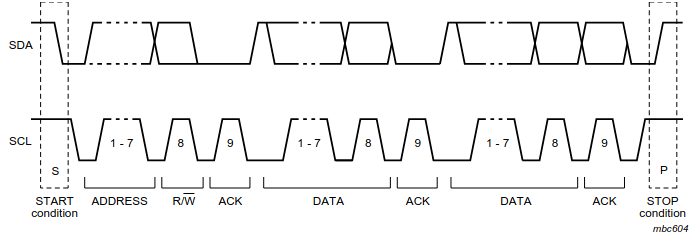
\includegraphics[width=0.95\textwidth]{figures/I2C_transaction.png}
    \end{center}
    \caption{I2C Communication transaction, SCL is the clock lane and SDA is the data lane.
        \textit{Image source: \href{https://www.nxp.com/docs/en/user-guide/UM10204.pdf}{I2C standard}}}\label{fig:I2C}
\end{figure}

The communication process works in the following way as seen in \cref{fig:I2C}:

\begin{enumerate}
    \item The master initiates the communication by lowering the data lane and
        keeping the clock lane up.

    \item The master sends a 7-bit address through the data lane to specify
        which device it wants to communicate with, followed by a read or write
        bit specifying which operation it wants to do.

    \item After receiving the message, the slave acknowledges (ACK) that it received
        the message by pulling down the data lane. If it is not ready, it will
        leave the data lane up (NAK).

    \item When the slave has responded, the master will send the data in 8-bit
        frames followed by an ACK/NAK bit.

    \item The transfer is finally stopped by releasing the data lane while the
        clock lane is up.
\end{enumerate}

In userspace Linux I2C is configured using \textit{ioctl} commands. This will
briefly be covered in \cref{section:v4l2}.

\section{History}
In this section we will cover the history of cameras on Linux.

In the early days cameras were quite simple, there effectively was just the
"press button" followed by receiving a picture. This process did not allow for
much customization. This was the case with most cameras such as webcams where
the camera sensors were "smart sensors". This meant that the cameras had a small
ISP integrated into them, they could do the processing internally. Even the
integrated laptop ones were just USB devices that spit out images. Linux had
initially had lacking support for this, but in the early 2000s Video For Linux
(V4L, later V4L2 for version 2) was developed. This covered most of the use
cases at the time. V4L grew organically over the years, it developed the
features that were needed as they were needed. This meant that there was no
large plan being executed, in turn the design that grew became a bad one
\footnote{Direct documentation on what was wrong with the API has not really
been written, this is based on a discussion with Laurent Pitchard}.
In 1998 Bill Dericks began the design and development of V4L2 which we have in
use today.

\begin{figure}
    \centering
    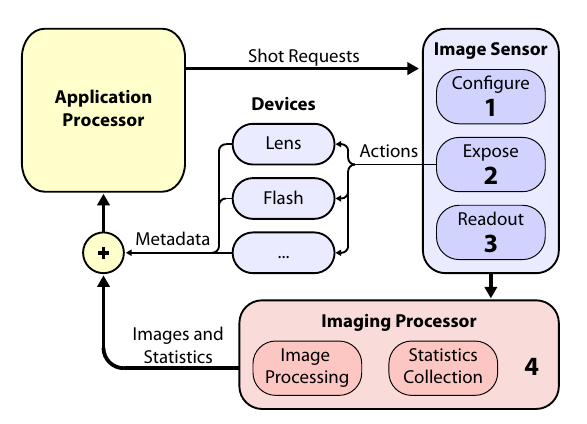
\includegraphics[width=0.48\textwidth]{figures/fcam_arch.png}
    \caption{Frankencamera archictecture~\cite{adams2010frankencamera}}
    \label{fig:fcam_api}
\end{figure}

In 2009 the Nokia N900 was released, this was a Linux based phone that was not
like most cameras at the time. It provided interfaces for customizing just
about everything. From ISPs to Image Processing Algorithms (IPAs), this meant
that the current way camera APIs worked was no longer maintainable. It
required that the application would manage everything, computing the
histograms, configuring the autocontrol etc.. While this was doable for a
company on the scale of Nokia at the time, it was not for anyone else. Enter
Frankencamera~\cite{adams2010frankencamera}; this was an effort at the time
to create an API that allowed the user to express the different options that
cameras needed. This effort was lead by Stanford and Nokia, it is what most
modern APIs are based on at a high level. It was built on top of V4L2,
providing a more user friendly API than the kernel drivers themselves.

Like its successors covored in~\cref{section:currentAPIs}, the Frankencam API
was a request based API. The idea with it was to allow for the user to control
the cameras very well. \cref{fig:fcam_api} shows the block diagram of how the
API worked. The application would request a capture, the sensor gets
reconfigured based on the request. After which it would capture the image with
which ever peripherals the user has and finally forward the image to the ISP.
The ISP then processes the image and gives it to the application along with the
metadata. This will look very similar to how modern APIs work which is covered
in~\cref{section:currentAPIs}.

Before Frankencam many camera APIs were stateful~\cite{experimentalCompPhot},
they only had one state that controlled the sensor. This meant that when you
wanted to capture multiple images with multiple settings the changes would take
effect at an unpredictable time in the future. While also adding latency to
manage the state internally, it also meant that you had to clear the capture
pipeline so that you could guarantee that the settings were correct. This was a
very complex process, though state was important; it was placed in the wrong
place. This lead to the creation of the request based API, where the
application would manage the state and the camera would simply accept requests.

